%-------------------------------------------------------------------------
\RequirePackage[]{lineno}
\documentclass[]{article}
\usepackage{caption}
\usepackage{times}
\usepackage{setspace}
\usepackage{longtable}
\usepackage{amsmath}
\usepackage{booktabs}
\usepackage{float}
\usepackage{mathpazo}
\usepackage{times}
\usepackage{tikz}
\usepackage{graphicx}
\usepackage[hmargin=2.25cm, vmargin=2cm, headheight=15.5pt]{geometry}
\usepackage{multirow}
\usepackage{tcolorbox}
\usepackage{multicol}
\usepackage{tabularx}
\usepackage{subfiles}
\usepackage{rotating}
\usepackage{lscape}
%\usepackage[hmargin=2.25cm, vmargin=2cm, headheight=15.5pt]{geometry}

\captionsetup[figure]{font=small}
\captionsetup[table]{font=small}

\usetikzlibrary{arrows,calc}
\geometry{margin=1in}

%\captionsetup{font=doublespacing, size= footnotesize}% Double-spaced float captions
\doublespacing
\DeclareCaptionJustification{double}{\DoubleSpacing}
% Reasonable page setup


\usepackage[]{natbib}
\bibpunct[; ]{(}{)}{;}{a}{,}{;}




\begin{document}


\subfile{sections/0_titlepage}
%\subfile{sections/1_introduction}
\section{Introduction}

The question of how genetic variation is maintained, despite the effects of selection and drift, continues to be central to the study of evolutionary biology \citep{walsh_evolution_2018}. Classical explanations include overdominance (heterozygote advantage) or frequency-dependent selection, but in the modern era of genomic data all patterns of elevated variation than expected under neutrality tends to be categorized broadly as balancing selection, regardless of the evolutionary mechanism \citep{mitchell-olds_which_2007}.  One of the evolutionary mechanisms coined under balancing selection is sexually antagonistc selection  which ouccrs when the direction of natural selection on traits or loci differs between the sexes \citep{connallon2018environmental}.

\textit{Paragraph about SAS theory and its limitations}

Sexually antagonist selection has been identified as a powerful engine of speciation, and more recently, as a mechanism that can mantain polymorphisms of otherwise dis-advantageous alleles in a population  \citep{connallon_evolutionary_2018, gavrilets2014sexual}. However, the effect of sexually antagonistic selection has been generally studied under strong assumptions such as homogeneous environments and stationary populations \citep{}. Few studies have explored the effect of sexually antagonistic selection on the maintenance of polymorphism with more realistic assumptions, such as \citet{connallon_evolutionary_2018} : description of their findings. However, the effect of environmental fluctuations without local adaptation have not been explored in the context of sexual conflict.

\textit{MCT as a way to study the effect of fluctuations in diversity maintenance}

Modern coexistence theory provides a useful conceptual framework that allows for quantifying the contribution of processes that shape ecological communities \citep{Chesson2000, mayfield2010opposing,hillerislambers2012rethinking,, Adleretal2018, petry2018competition}. At its core, modern coexistence theory is built on models of pairwise interactions among competitors, and the coexistence of these competitors depend on the relative importance of stabilizing mechanisms and fitness differences \citep{Chesson2000, chesson2000general, chesson2003quantifying, letten_linking_2017, Adleretal2018, barabas_chessons_2018}. Stabilizing mechanisms cause a species to buffer its own growth when at high density more than it buffers growth of a competitor, and fitness differences describe differences in competitive abilities or growth rates among species \citep{Chesson2000,chesson2003quantifying, levine2009importance}. Many mechanisms can lead to stabilizing mechanisms such as complimentary resource use \citep{tilman1994competition}, differential responses to spatial and temporal environmental variation \citep{chesson1981environmental, angert2009functional}, and species-specific effects of natural enemies \citep{Paine1966, Paine1969, Connell1972,janzen1970herbivores}. Fitness differences reflect differences in resource use and can establish competitive hierarchies among species \citep{godwin2020empiricist}. When stabilizing mechanisms become sufficiently strong to overcome fitness differences, long-term coexistence is possible \citep{Chesson2000}.

\textit{Paragraph that links MCT and evolution}

In this paragrph we introduce the idea that polymorphism is equal to coexistence from a MCT theory perspective. We also introduce fluctuations in population sizes and fitness values as mechanisms that could enhance the role of SAS and how MCT could help distinguish their effect with the partition of growth rates (Ellner)

% directly from slack
\textit{Paragraph about what we do in this paper}


Here we seek to explicitly apply recent theoretical and analytical advances in coexistence theory to the question of how genetic variation is maintained. We aim to quantify the relative importance of different types of fluctuations to overall stable coexistence, or to exclusion of alleles. We extended a conceptualisation of MCT \citep{ellner2016quantify,ellner_expanded_2019} to examine how fluctuations in fitness differences, fluctuations in population sizes, and their interactions can stabilize or hinder coexistence. In particular we examined :

\begin{itemize}
	\item Can fluctuations in population sizes and fitness differences allow sexually antagonistic allleles to coexist when differences in their fitness would typically not allow them to?
	%\item What is the effect of different types of fluctuations in the proportion of parameter space that allows alleles to coexist?
	\item What is the relative contribution of different types of fluctuations that allow each allele to invade ?
\end{itemize}

\clearpage
\section{Methods}

We used an extended version of MCT to quantify the contribution of fluctuations in population sizes and fitness values in the coexistence of sexually antagonistic alleles. As a baseline, we first present the evolutionary consequences of sexually antagonistic selection in constant environments. Then, we present how the dynamics that describe the changes in alleles' frequencies after one generation can be expressed in terms of growth rates, a necessary condition to analyses done using MCT. We continue by giving a brief explanation of how MCT decomposes and compares population growth rates to understand the relative contribution of abiotic and biotic variables to coexistence and show how the growth rates of antagonistic alleles can be examined through this lens. Finally, we apply our framework by simulating different scenarios where we allowed population sizes, fitness values, both, or neither to vary, to calculate the contribution of each of these fluctuations in the coexistence of alleles across the parameter space of sexually antagonist selection.


\subsection*{Evolutionary dynamics of sexually antagonistic alleles}

 Most population genetic models of sex-dependent selection consider evolution at single, biallelic  loci with frequency and density independent effeccts on the relative fitness of females and males \citep{wright1942statistical,kidwell1977regions, immler2012ploidally}. Consider a locus with two alleles, $j$ and $k$, that affect fitness in the haploid state.  Assume allele $j$ always has a high fitness in females ($w_{jf} = 1$), but has variable fitness in males ($w_{jm}$), and allele $k$ always has a high fitness in males ($w_{km} = 1$), but has variable fitness in females ($w_{kf}$). The selection against males is therefore $S_{m}= 1 - w_{jm}$, and the selection against females is $S_{f}= 1 - w_{kf}$ . Selection mantains both alleles in the population under the condition that:

 \begin{equation}
\frac{S_{m}}{1+S_{m}} < S_{f} < \frac{S_{m}}{1-S_{m}}
\label{selection}
 \end{equation}

\citep{kidwell1977regions,pamilo1979genic,connallon_evolutionary_2018}. These inequalities can be used to calculate the proportion of parameter space (within the range $ 0 < S_{m}, S_{f} < 1$) that leads to polymorphism of sexually antagonistic alleles: in $\approx 0.31$ of the parameter space allele $j$ will be fixed, in another $\approx 0.31$ of the parameter space allele $k$ will be fixed, and in $\approx 0.38$ of the parameter space polymorphism or coexistence of alleles can be maintained. However, most of the models used to explore the evolutionary dynamics of sexual antagonism assume constant population sizes and homogeneous environments \citep{kidwell1977regions,pamilo1979genic}. In constant environments, the maintenance of polymorphism of sexually antagonistic alleles is solely determined by the values of $S_{m}$ and $S_{f}$. If fluctuations in population sizes or fitness values can promote the coexistence of sexually antagonistic alleles, it would be reflected in an increase of the proportion of the parameter space where polymorphism is maintained.


\subsection*{Population dynamics of sexually antagonistic alleles}

Although the evolutionary dynamics of sexually antagonistc selection are often explored though changes in alleles' frequencies, MCT requires population dynamics to be expressed as growth rates. Consider a population that has discrete generations, and that is subject to the previously described sexual antagonism between allele $j$ and $k$. The proportion of each allele in each sex at the beginning of a life-cycle is given by:
\begin{equation}
    p_{jm}= \frac{n_{jm}}{N_{m}}
    \label{first_pop}
\end{equation}
\begin{equation}
    p_{jf}= \frac{n_{jf}}{N_{f}}
\end{equation}
\begin{equation}
    p_{km}= \frac{N_{m}-n_{jm}}{N_{m}}
\end{equation}
\begin{equation}
    p_{kf}= \frac{N_{f}-n_{jf}}{N_{f}}
\end{equation}
where $N_m$ and $N_f$ are the numbers of males and females in a population, $n_{jf}$ is the number of females $f$ with allele $j$, and $n_{jm}$ is the number of males $m$ with allele $j$.

If the individuals in the population mate at random before selection occurs, the proportion of offspring with allele $j$ after mating can be expressed as:
%Convert frequencies to counts (abundances) to move to coexistence framework. The explicit calculation of $p'_{j}$ prime from random mating what selection acts on yields
\begin{equation}
   p'_{j}= \frac{n_{jf}}{N_{f}} \frac{n_{jm}}{N_{m}} + \frac{1}{2} \frac{n_{jf}}{N_{f}} \frac{(N_{m}-n_{jm})}{N_{m}} +\frac{1}{2}
   \frac{(N_{f}-n_{jf})}{N_{f}} \frac{n_jm}{N_{m}} \,,
\end{equation}
which upon rearranging and simplifying can be written as:
\begin{equation}
   p'_{j}= \frac{(N_{m}n_{jf}+ N_{f}n_{jm})}{2 N_{f}N_{m}} \,.
   \label{pprime}
\end{equation}

Selection acts upon these offspring in order to determine the allelic frequencies in females and males in the next generation. As an example, if $w_{jf}$ is the fitness of allele $j$ in females $f$, then the proportion of females with allele $j$ after selection is:
\begin{equation}
   p^{\prime}_{jf}= \frac{n'_{jf}}{N'_{f}} = \frac{p'_{j}w_{jf}}{p'_{j}w_{jf}+ (1-p'_{j})w_{kf}}
\end{equation}

The logarithmic growth rate of $j$ in females, is given by the number of females with allele $j$ after selection, divided by the original number of females carrying allele $j$:



\begin{equation}
    r_{jf} = \ln \left( \frac{n'_{jf}}{n_{jf}} \right)
    \label{canonical}
\end{equation}
%Which after substitution can be expressed as:

%\begin{equation}
%  r_{jf} = \ln \left[ \frac{N'_{f}}{n_{jf}} \left( \frac{(N_{m}n_{jf}+ N_{f}n_{jm})w_{jf}}{(N_{m}n_{jf}+ N_{f}n_{jm})w_{jf} + (2N_{m}N_{f}-N_{m}n_{jf}-N_{f}n_{jm})w_{kf}} \right) \right] \,.
%\label{usefulequation}
%\end{equation}

An equivalent expression for the per capita growth rate of allele $j$ in males $m$ can be obtained by exchange $f$ for $m$ across the various subscripts in this expression.

When placed in the canonical form, the growth rate of allele $j$ in females $f$ is given by Eqn~\ref{canonical}. However, allelic coexistence in a sexual population is ultimately influenced by growth and establishment of an allele across both sexes. Therefore, the full growth rate of allele $j$ across the entire population of females \emph{and} males is given by
\begin{equation}
    r_{j} = \ln \left(  \frac{n_{jf}e^{r_{jf}}}{n_{jf} + n_{jm}}   +  \frac{n_{jm}e^{r_{{jm}}}}{n_{jf} + n_{jm}}  \right) \,.
    \label{full}
\end{equation}

%We can substitute using Eq.~\ref{usefulequation} and the corresponding expression for the growth rate of allele $j$ in males $m$ to obtain:
%\begin{eqnarray}
%        r_{j} =  \ln \left(  \frac{n_{jf}}{n_{jf}+ n_{jm} } \left[ \frac{N'_{f}}{n_{jf}} \frac{(N_{m}n_{jf}+ N_{f}n_{jm})w_{jf}}{(N_{m}n_{jf}+  N_{f}n_{jm})w_{jf} + (2N_{m}N_{f}-N_{m}n_{jf}-N_{f}n_{jm})w_{kf}} \right] \right. \nonumber \\
%        + \left. \frac{n_{jm}}{n_{jf} + n_{jm}} \left[\frac{N'_{m}}{n_{jm}}
%    \frac{(N_{m}n_{jf}+ N_{f}n_{jm})w_{jm}}{(N_{m}n_{jf}+ N_{f}n_{jm})w_{jm} + (2N_{m}N_{f}-N_{m}n_{jf}-N_{f}n_{jm})w_{km}}  \right] \right)
%\end{eqnarray}
% for some reason this last parenthesis has decided not to be big
% you cannot have autosized parentheses the span across lines. you need to add a dummy sizing element \left. to trick it to behave


%Which simplifies to:

%\begin{eqnarray}
%    r_{j} = \ln \left( \frac{N'_{f}}{n_{jf}+ n_{jm}} \left[ \frac{(N_{m}n_{jf}+ N_{f}n_{jm})w_{jf}}{ (N_{m}n_{jf}+ N_{f}n_{jm})w_{jf} + (2N_{m}N_{f} - N_{m}n_{jf}- N_{f}n_{jm})w_{kf}  } \right] \right)\\
%    + \ln \left(1 + \frac{N'_{m}}{N'_{f}} \frac{w_{jm}}{w_{jf}} \left[ \frac{ (N_{m}n_{jf} + N_{f}n_{jm})w_{jf} + (2 N_{m}N_{f}- N_{m}n_{jf}- N_{f}n_{jm} )w_{kf}}{(N_{m}n_{jf} + N_{f}n_{jm})w_{jm} + (2N_{m}N_{f}- N_{m}n_{jf}- N_{f}n_{jm})w_{km} } \right] \right)
%    \label{rj}
%\end{eqnarray}

We show the full substitution of Eqns.\ref{canonical} and \ref{full} in the Supporting Information. Equivalently, there exists an expression for $r_{k}$. This re-formulation of changes in alleles frequencies to growth rates does not change the results of selection given by Eqn.~\ref{selection}. The fitness values, and consequently the values of the selection coefficients, will determine whether or not an allele is fixed in the population, which would would be reflected in positive growth rates.

\subsection*{Growth rate decomposition using MCT}

Modern coexistence theory has shown that coexistence is stabilized by mechanisms that give species a population growth rate advantage over other species when they become rare \citep{chesson_stabilizing_1982, chesson2003quantifying, barabas_chessons_2018}. Typically, the other species are at their \textit{resident} state, or remain at steady-state abundances, while the rare species is called the \textit{invader}. In the context of alleles in a population, an allele is an \textit{invader} when a mutation occurs that introduces that allele into the population (e.g., if in a population with only $k$ alleles, a random mutation made one individual carry the $j$ allele). Given sexually antagonistic selection, each allele has two pathways of invasion, depending on where the mutation occurs: females or males. If an alleles' \textit{invasion growth rate} (or the average instantaneous population growth rate when rare) is positive, it buffers it against extinction, maintaining its persistence in the population.  Coexistence, or polymorphism, occurs when all of the alleles in a population have positive invasion growth rates.

MCT provides an analytical framework to decompose each species' , or in our case allele's, invasion growth rates into a sum of terms for the effects of different factors, such as abiotic and biotic fluctuations, and then compare invader and residents term by term \citep{ellner_expanded_2019}. Mechanisms that stabilize coexistence can help whichever allele is rare, or it can hurt whichever allele is common. Therefore, to understand the role of each mechanism, it is necessary to compare how it affects invader \textit{and} resident growth rates. MCT uses Taylor series expansion to do this decomposition and comparison (a detailed review can be found in \citet{barabas_chessons_2018}). We present an analytical approach, using classic MCT, to understand the relative contributions of fluctuation in population sizes and fitness values to each alleles' growth rate as an invader in the Supporting Information.

Our general solution using Taylor series expansion, however, is not easily interpreted and soon becomes mathematically untraceable (Supporting Information). Therefore, we turned towards an extension of MCT \citep{ellner_expanded_2019} that provides the flexibility to analyze the contributions of different processes to coexistence using \textit{functional decomposition}. This approach applies to any collection of two or more processes, mechanisms, or species differences affecting population growth rate \citep{ ellner2016quantify, ellner_expanded_2019}, and has been used to show the relative contribution of variable temperature and silicate to the coexistence of algal species \citep{ellner2016quantify} and to quantify the relative importance of environmental fluctuations and variation in predator abundances to the coexistence of intertidal species \citep{shoemaker2020}.

The functional decomposition approach focuses on any biotic or abiotic variables affecting a population growth rate. It consists of breaking up the average growth rate of each species into a null growth rate in the absences of all selected variables, a set of main effect terms that represent the effect of adding only one variable, and a set of two--way interaction terms representing the effect of adding each possible pair of features \citep{ellner_expanded_2019}.

For example, a population growth rate $r$ of a population $i$ can be function of abiotic fluctuations $X$, and biotic fluctuations $Y$:

\begin{equation}
   r_{i}(X,Y) = \mathcal{E}^{0} + \mathcal{E}^{X}+ \mathcal{E}^{Y}+ \mathcal{E}^{XY}
   \label{functional_decomp}
\end{equation}

Where $\mathcal{E}^0$ is defined as the null growth rate when the abiotic and biotic variables are set to their averages. Terms with superscripts represent marginal effects of letting all superscripted variables vary while fixing all the other variables at their average values. For example, the term $\mathcal{E}^X$ expresses the contribution of the variable $X$ to a growth rate when $Y$ is at its average, without the contribution when both variables are set to their averages :

\begin{equation}
  \mathcal{E}^{X} = r_{i}(X,\overline{Y}) - \mathcal{E}^{0}
\end{equation}


Averaging both sides of ~\ref{functional_decomp} gives a partition of the average population growth rate of invading into the variance--free growth rate, the main effects of variability in $X$, the main effects of variability in $Y$, and the interaction between variability in $X$ and $Y$

\begin{equation}
    \overline{r}_{i}= \mathcal{E}^{0} + \overline{\mathcal{E}}^{X}+ \overline{\mathcal{E}}^{Y}+ \overline{\mathcal{E}}^{XY}
   \label{functional_decomp_2}
\end{equation}

In the case of antagonistic alleles we previously introduced, the functional decomposition of both alleles' growth rates is a function of four variables: the number of males in the population ($N_{m}$), the number of females in the population ($N_{f}$), the fitness of allele $j$ in males ($w_{jm}$), and the fitness of allele $k$ in females ($w_{kf}$).The implementation and interpretation of the functional decomposition of the growth rates of each allele are identical to each other. For simplicity,  we present the full functional decomposition of the growth rate of allele $j$ in Table \ref{tab:EllnerRs}, as well as a brief description of the meaning of each term.

The functional decomposition approach further requires the \textit{comparison} of each term, to understand if how it affects invader and residents. Suppose Eqn.~\ref{functional_decomp_2} represents the functional  decomposition of an invader $i$. An analogue decomposition of a resident $r$ growth rate would be given by $\overline{r}_{r}$, which being at steady state means $\overline{r}_{r}=0$. We therefore can express:


\begin{equation}
    \overline{r}_{i}= \overline{r}_{i} - \overline{r}_{r} = \Delta^{0} + \Delta^{X}+  \Delta^{Y}+ \Delta^{XY}
   \label{functional_decomp_3}
\end{equation}

Where each $\Delta$ term denotes the difference between the invader and resident terms. For example $\Delta^{0}$  is the difference in population growth rates at mean values of $X$ and $Y$, $\Delta^{X}$ is the difference in the main effects of variability in $X$ between invader and resident, and so on. This comparison allows decomposing each species' growth rate when rare into its mechanistic contributions. Mechanisms may have minimal effects, a destabilizing effect (a negative contribution to a species' growth rate when rare), or a stabilizing effect (a positive contribution to a species' growth rate when rare) \citep{shoemaker2020}.

In the case of antagonistic alleles, each term in Table \ref{tab:EllnerRs} can be compared to an analogue one of the other allele as a resident. For example, if allele $j$ is the invader and allele $k$ is the resident, the difference in invader and resident growth rates when the male population varies is given by:


\begin{equation}
\Delta^{Nm}_{j}= \overline{\mathcal{E}}^{Nm}_{j} - \overline{\mathcal{E}}^{Nm}_{k}
\label{delta}
\end{equation}

If $\Delta^{Nm}_{j}$ is positive, then fluctuations in the male population benefit allele $j$ when it is rare more than what they benefit $k$ as a resident. If $\Delta^{Nm}_{j}$ is negative, then fluctuations benefit $k$ as a resident more than $j$ as an invader, and if it is minimal, then fluctuations have an equal effect in $j$ and $k$. However, coexistence occurs when both alleles, when rare, can invade a population, so for fluctuations in males to have a stabilizing effect, they should be positive for $\Delta^{Nm}_{j}$ and $\Delta^{Nm}_{k}$

\subsection*{Simulations}

Our simulations consisted of performing  invasion simulations of both alleles invading separetly, allowing population sizes and fitness values to fluctuate, across the parameter space of sexually antagonistic selection. Then, we used the functional decomposition approach to decompose and compare the relative contribution of fluctuations to the coexistence of sexually antagonistic alleles. For simplicity, we first present our approach focusing on a fixed point in the parameter space.

\vspace{5mm}
\noindent\textbf{Timeseries}

For a determined value of $w_{jm}$ and $w_{kf}$, we first created a timeseries which projected our population model (Eqns.~\ref{first_pop} to \ref{full}) 500 timesteps. To generate the initial population, we used initial values of $N_{m}$ and $N_{f}$  of 200 individuals each, and equal frequencies of allele $j$ and allele $k$ in each sex. Throughout each timestep, we controlled how much populations sizes ($\sigma_{g}$), and fitness values ($\sigma_{w}$) varied, as well their correlations ($\rho_{g}$ and $\rho_{w}$). We show the full range of parameter values we used to introduce fluctuations in Table \ref{tab:fluctuations}.

To introduce fluctuations in fitness values, following the appoach of  \citet{shoemaker2020}, we first generated a matrix of uncorrelated random viables using a normal distribution with a mean of zero and a standard deviation of one, for both of the fluctuating fitness values. Each matrix had two rows, and the same number of columns as number of timesteps in our simulations. Following this, we used the Cholesky factorisation of the variance-covariance matrix:


\begin{equation}
C_{w} = \begin{bmatrix}
\sigma_{w}^{2} & \rho_{w} \sigma_{w}^{2} \\
\rho_{w} \sigma_{w}^{2} & \sigma_{w}^{2}
\end{bmatrix}
\label{covmat}
\end{equation}

to create random normally distributed  rates of change for each fitness value, by multiplying Eqn.~\ref{covmat} by the corresponding matrix of uncorrelated random variables. Finally, we calculated the value of $w_{jm}$ and $w_{kf}$ to be used in each timestep, by elevating their fixed value to the corresponding rate of change. We imposed an upper bound to the values $w_{jm}$ and $w_{kf}$ at one since the parameter space of selection ranges from zero to one.

We introduced fluctuations in population sizes similar to fluctuations in fitness values: we created a matrix of uncorrelated random variables and performed a Cholesky factorisation of the corresponding variance-covariance matrix. Then, we calculated a new population size of males and females by adding to the mean value of $N_{m}$ and $N_{f}$, the corresponding value of the product of the variance-covariance matrix and the correspoing matrix of uncorrelated random variables. We bounded how much population sizes could fluctuate so there were no negative population sizes since that would not be biologically plausible. Following this, we calculated the rate of change for $N_{m}$ and $N_{f}$ for each timestep. Finally, we calculated the values of $N_{m}$ and $N_{f}$ to be used at each timestep of our simulation by elevating their mean value to the corresponding rate of change.

\vspace{5mm}
\noindent\textbf{Invasion simulations}

We used the timeseries described previously to perform invasion simulations of both alleles. Each allele could invade via two different pathways: males and females. We explored all of the combinations of each allele invading through a different pathway (e.g., allele $j$ invading through males, and allele $k$ invading through females, and so on). Therefore, for every point in the parameter space of sexually antagonistic selection, we explored four different types of invasion.

For each timestep in the timeseries, we performed simulations of the two alleles invading separetly via their respective pathway. To simulate invasion, we set the initial values of the invading allele to one individual, while the resident allele was set to the correspoing value of the timeseries, and we projected forward one generation. For example, if allele $j$ was invading via males, then we would set $n_{jm} = 1$ and $n_{jf}= 0$, while the allele $k$ would be the resident. The abundance of the resident was determined by the timestep $t$ of the timeseries. After one generation, we calculated the logarithmic growth rate of \textit{j} allele invading as:

\begin{equation}
r_{j} =	\ln \left ( \frac{n_{jm,t +1 } + n_{jf,t+1}}{1} \right )
\label{invader}
\end{equation}

Correspondingly, the logarithmic growth rate of the \textit{k} allele as a resident would be given by:
\begin{equation}
r_{k} =	\ln \left ( \frac{ n_{km,t+1} + n_{kf,t+1} }{ n_{km,t} + n_{kf,t}  } \right )
\label{resident}
\end{equation}

We treated each timestep of the timeseries independently, so we performed 500 invasion simulations, one for each timestep. Then, we calculated the mean invasion growth rate as the average of the 500 invasion growth rates, and the mean reasident growth rate as the average of the 500 resident growth rates. We determined alleles to be coexisting if both of them, invading via their respective pathway, had positive  mean invasion growth rates, which is also called the mutual invasibility criterion.

\vspace{5mm}
\noindent\textbf{Functional decompostion}

To understand the relative contribution of fluctuations in population sizes and fitness values, we applied the functional decomposition framework we previously described. To do so, we performed another set of invasion simulations of each allele invading via its corresponding pathway, but setting all of the  fluctuating variables to their means. Then, we calculated invader and resident mean growth rates as previously described (e.g., Eqns.\ref{invader} and \ref{resident}). When every variable was set to its mean, the average invasion and resident growth rate was equal to $\mathcal{E}^{0}$.

Building upon this baseline, we performed another set of invasion simulations, but this time allowing variables to fluctuate one by one, to capture their main effects, and jointly, to capture their interactions. Then, we  caclulated the corresponding values of each $\mathcal{E}$ term, as shown in Table \ref{tab:EllnerRs}. For simplicity, we only show the functional decomposition of $j$ as an invader in Table \ref{tab:EllnerRs}, however, the functional decomposition of $k$ as an invader is identical.  This approach allowed us to capture the contribution of fluctuations to invader and resident growth rates, which we did for each allele invading a different pathway.

Having done the decomposition of invader and resident growth rates, we continued to do the invader-resident comparisons to calculate $\Delta$ values (e.g.,~\ref{delta}). For each allele invading via a different pathway, we calculated 16 $\Delta$ values, one for each one of the $\mathcal{E}$ terms. However, since the magnitude of each one of these values could vary considerably, to make them comparable, we normalized each $\Delta$ value by dividing it by the lenght of the $\boldsymbol{\Delta}$ vector. For example, the normalized value of Eqn.~\ref{delta} would be given by:

\begin{equation}
  \Delta^{Nm*}_{j}= \frac{\Delta^{Nm}_{j}}{\sqrt{
    \sum\limits_{i=1}^{16} (\boldsymbol{\Delta_{i}})^{2} }}
\end{equation}

This normalization bounded $\Delta$ values from $-1$ to $1$.

\vspace{5mm}
\noindent\textbf{The parameter space of sexually antagonist selection}

To evaluate if fluctuations in fitness values and population sizes allow sexually antagonistic alleles to coexist when their fitness values would typically not allow them to, we applied the approach presented so far to the whole parameter space of selection  ($ 0 < S_{m}, S_{f} < 1$). To do so, we partinioned the parameter space in 2500 parts, each one a combination of different $w_{jm}$ and $w_{kf}$ values. For each parameter combination, we  separetly calculated each allele's mean invasion growth rate when invading through males and females, as well as its functional decomposition. Then, we determined coexistence outcomes using the mutual invasibility criterion. Finally, we calculated the proportion of the parameter space that allowed alleles to coexist, for each allele invading via a different sex.

We explored all of  the combinations of low ($\sigma_{w} = 0.1$ and $\sigma_{g}=1$), intermediate (($\sigma_{w} =  0.3$ and $\sigma_{g}=10$)) and high fluctuations ($\sigma_{w} = 0.7$ and $\sigma_{g}=30$) in fitness values and population sizes, with different extents of correlations between fluctuations (Table \ref{tab:fluctuations}).  As a control simulation, we set $\sigma_{w}= 0.001$ and  $\sigma_{g}=0.001$, with no correlation between fluctuations. For each one of the factorial combinations of $\sigma_{g}$, $\sigma_{w}$, $\rho_{g}$ and $\rho_{w}$ (Table \ref{tab:fluctuations}), we performed invasion simulations across the parameter space of selection. We did three replicates per parameter combination, which resulted in 432 simulations.


\clearpage
\subsection*{Results}



\clearpage
\subsection*{Figures and tables }




\begin{table}[h]
\fontsize{7}{12}\selectfont % the spacing on this is rough
    \centering
      \caption{Functional decomposition of the growth rate of allele $j$. Need to get rid of the sums and $m$ because we are only presenting $j$. As well to add an overbar over rj. }
  \resizebox{\textwidth}{!} {\begin{tabular}{l|l|l}
  \toprule
        Term & Formula & Meaning \\
        \hline
         $\mathcal{E}^{0}_{j}$ & $\overline{r_{j}} (\overline{N_{m}}, \overline{N_{f}}, \overline{w_{jm}}, \overline{w_{kf}})$ & Growth rate at mean population size and fitness values. \\


         $\overline{\mathcal{E}}^{N_{m}}_{j}$ & $\overline{r}_{j}(N_{m} \overline{N_{f}}, \overline{w_{jm}}, \overline{w_{kf}}) - \mathcal{E}^{0}_{j} $ & Main effect of fluctuations in $N_{m}$\\

         $\overline{\mathcal{E}}^{N_{f}}_{j}$ & $ \overline{r_{j}}( \overline{N_{m}}, N_{f},\overline{w_{jm}}, \overline{w_{kf}}) - \mathcal{E}^{0}_{j}$ & Main effect of fluctuations in $N_{f}$ \\

        $\overline{\mathcal{E}}^{w_{jm}}_{j}$ & $ \overline{r_{j}}(\overline{N_{m}}, \overline{N_{f}}, w_{jm}, \overline{w_{kf}}) - \mathcal{E}^{0}_{j}$& Main effect of fluctuations in $w_{jm}$\\

        $\overline{\mathcal{E}}^{w_{kf}}_{j}$ & $ \overline{r_{j}}(\overline{N_{m}}, \overline{N_{f}}, \overline{w_{jm}}, w_{kf})- \mathcal{E}^{0}_{j}$ & Main effect of fluctuations in $w_{kf}$\\

        $\overline{\mathcal{E}}^{N_{m},N_{f}}_{j}$ & $ \overline{r_{j}}(N_{m}, N_{f}, \overline{w_{jm}}, \overline{w_{kf}})- [\mathcal{E}^{0}_{j} +\overline{\mathcal{E}}^{N_{m}}_{j}+\overline{\mathcal{E}}^{N_{f}}_{j}]$ & Interaction of fluctuations in $N_{m}$ and $N_{f}$\\

        $\overline{\mathcal{E}}^{w_{jm},w_{kf}}_{j}$ & $ \overline{r_{j}}(\overline{N_{m}}, \overline{N_{f}}, w_{jm}, w_{kf})- [\mathcal{E}^{0}_{j} +\overline{\mathcal{E}}^{w_{jm}}_j+\overline{\mathcal{E}}^{w_{kf}}_{j}]$ & Interaction of fluctuations in $w_{jm}$ and $w_{kf}$ \\

        $\overline{\mathcal{E}}^{N_{m}w_{jm}}_{j}$ & $\overline{r_{j}}(N_{m}, \overline{N_{f}}, w_{jm}, \overline{w_{kf}})- [\mathcal{E}^{0}_{j} +\overline{\mathcal{E}}^{N_{m}}_j+\overline{\mathcal{E}}^{w_{jm}}_{j}]$  & Interaction of fluctuations in $N_{m}$ and $w_{jm}$ \\


        $\overline{\mathcal{E}}^{N_{m}w_{kf}}_{j}$& $ \overline{r_{j}}(N_{m}, \overline{N_{f}}, \overline{w_{jm}}, w_{kf})- [\mathcal{E}^{0}_{j} +\overline{\mathcal{E}}^{N_{m}}_j+\overline{\mathcal{E}}^{w_{kf}}_{j}]$ & Interaction of fluctuations in $N_{m}$ and $w_{kf}$\\


        $\overline{\mathcal{E}}^{N_{f}w_{jm}}_{j}$& $\overline{r_{j}}(\overline{N_{m}}, N_{f}, w_{jm}, \overline{w_{kf}})- [\mathcal{E}^{0}_{j} +\overline{\mathcal{E}}^{N_{f}}_j+\overline{\mathcal{E}}^{w_{jm}}_{j}]$ & Interaction of variation in $N_{f}$ and $w_{jm}$ \\

        $\overline{\mathcal{E}}^{N_{f}w_{fk}}_{j}$& $ \overline{r_{j}}(\overline{N_{m}}, N_{f}, \overline{w_{jm}}, w_{kf})- [\mathcal{E}^{0}_{j} +\overline{\mathcal{E}}^{N_{f}}_j+\overline{\mathcal{E}}^{w_{kf}}_{j}]$ & Interaction of fluctuations $N_{f}$ and $w_{kf}$ \\

 %%%%%%%%%triplicate terms

        $\overline{\mathcal{E}}^{N_{m}w_{jm}w_{fk}}_{j}$& $ \overline{r_{j}}(N_{m}, \overline{N_{f}}, w_{jm}, w_{kf})- [\mathcal{E}^{0}_{j} +\overline{\mathcal{E}}^{N_{m}}_{j}+\overline{\mathcal{E}}^{w_{jm}}_j+\overline{\mathcal{E}}^{w_{kf}}_{j}]$  & Interaction of fluctuations in $N_{m}$, $w_{jm}$, and $w_{kf}$ \\

      $\overline{\mathcal{E}}^{N_{f}w_{jm}w_{fk}}_{j}$& $ \overline{r_{j}}(\overline{N_{m}}, N_{f}, w_{jm}, w_{kf})- [\mathcal{E}^{0}_{j} +\overline{\mathcal{E}}^{N_{f}}_{j}+\overline{\mathcal{E}}^{w_{jm}}_j+\overline{\mathcal{E}}^{w_{kf}}_{j}]$ & Interaction of fluctuations in $N_{f}$, $w_{jm}$, and $w_{kf}$ \\

      $\overline{\mathcal{E}}^{N_{m}N_{f}w_{jm}}_{j}$& $ \overline{r_{j}}(N_{m}, N_{f}, w_{jm}, \overline{w_{kf}})- [\mathcal{E}^{0}_{j} +\overline{\mathcal{E}}^{N_{m}}_{j}+\overline{\mathcal{E}}^{N_{f}}_{j}+\overline{\mathcal{E}}^{w_{jm}}_j]$ & Interaction of variation in $N_{m}$, $N_{f}$, and $w_{jm}$ \\



      $\overline{\mathcal{E}}^{N_{m}N_{f}w_{fk}}_{j}$& $ \overline{r_{j}}(N_{m}, N_{f}, \overline{w_{jm}}, w_{kf})- [\mathcal{E}^{0}_{j} +\overline{\mathcal{E}}^{N_{m}}_{j}+\overline{\mathcal{E}}^{N_{f}}_{j}+\overline{\mathcal{E}}^{w_{kf}}_j]$ & Interaction of fluctuations in $N_{m}$, $N_{f}$, and $w_{kf}$ \\

%%%%%%%last part
$\overline{\mathcal{E}}^{N_{m}N_{f}w_{jm}w_{fk}}_{j}$&  $ \overline{r_{j}}(N_{m}, N_{f}, w_{jm}, w_{kf})- [\mathcal{E}^{0}_{j} +\overline{\mathcal{E}}^{N_{m}}_{j}+\overline{\mathcal{E}}^{N_{f}}_{j}+\overline{\mathcal{E}}^{w_{jm}}_j+\overline{\mathcal{E}}^{w_{kf}}_j$] & Interaction of variation in $N_f$, $N_m$, $w_{jm}$, and $w_{kf}$ \\



         \bottomrule
    \end{tabular}}
    \label{tab:EllnerRs}
\end{table}



\begin{table}[h]
\fontsize{10}{18}\selectfont
\centering
\caption{This is a caption}
\begin{tabular}{@{}llll@{}}
\toprule
Parameter                    & Values                    & Description                                   &  \\ \midrule
$\sigma_{w}$ & 0.001, 0.1, 0.3, 0.5, 0.7, 0.9 & Effect size of fluctuations in fitness values &  \\
$\sigma_{g}$ & 0.001, 1, 10, 20, 30, 50 & Effect size of fluctuations in population sizes                                              &  \\
$\rho_{w}$  &  -0.75, 0, 0.75                         &   Correlation between fluctuations in fitness values                                            &  \\
$\rho_{g}$  &   -0.75, 0, 0.75                        &  Correlation between fluctuation in population sizes                                             &  \\ \bottomrule
\end{tabular}
\label{tab:fluctuations}
\end{table}



\begin{figure}[h]
  \centerline{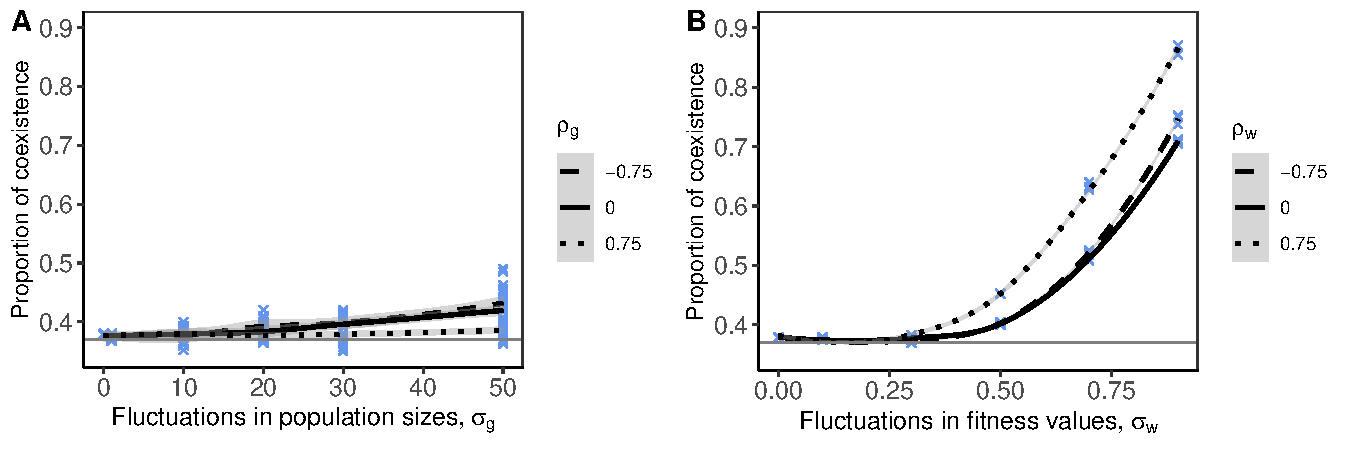
\includegraphics[width=1\textwidth]{fluctuations.pdf}}
  \caption{ }
    \label{fig:fitness_deltas}
\end{figure}




\clearpage
\bibliographystyle{ecology_letters}
\bibliography{coexistence.bib}

\end{document}
